\documentclass[12pt,a4paper]{article}

\usepackage[a4paper,width=160mm,top=25mm,bottom=25mm]{geometry}

\usepackage{fancyhdr}
\pagestyle{fancy}
\fancyhf{}
\fancyhead[EL]{\nouppercase\leftmark}
\fancyhead[OR]{\nouppercase\rightmark}
\fancyhead[ER,OL]{\thepage}

\usepackage{url}
\usepackage[hidelinks]{hyperref}

\renewcommand{\linethickness}{0.05em}
\usepackage[brazil]{babel}   
\usepackage{titlesec}
\newcommand{\sectionbreak}{\clearpage}


\title{Processando a Informação: um livro prático de programação independente de linguagem 
\\\large\vspace{2cm}
Rogério Perino de Oliveira Neves 
\\\vspace{5mm}
Francisco de Assis Zampirolli
\\\large\vspace{2cm}
EDUFABC
\\ \url{editora.ufabc.edu.br}
\\\Huge\vspace{3cm}
Notas de Aulas inspiradas no livro
\\\Large\vspace{1cm}
Utilizando a(s) Linguagem(ns) de Programação: 
\\\Huge\vspace{1cm}
C
\\\large\vspace{1cm}
Exemplos adaptados para Correção Automática no Moodle+VPL
\vspace{2cm}}
\author{Francisco de Assis Zampirolli\vspace{1cm}}


    \usepackage[breakable]{tcolorbox}
    \usepackage{parskip} % Stop auto-indenting (to mimic markdown behaviour)
    

    % Basic figure setup, for now with no caption control since it's done
    % automatically by Pandoc (which extracts ![](path) syntax from Markdown).
    \usepackage{graphicx}
    % Maintain compatibility with old templates. Remove in nbconvert 6.0
    \let\Oldincludegraphics\includegraphics
    % Ensure that by default, figures have no caption (until we provide a
    % proper Figure object with a Caption API and a way to capture that
    % in the conversion process - todo).
    \usepackage{caption}
    \DeclareCaptionFormat{nocaption}{}
    \captionsetup{format=nocaption,aboveskip=0pt,belowskip=0pt}

    \usepackage{float}
    \floatplacement{figure}{H} % forces figures to be placed at the correct location
    \usepackage{xcolor} % Allow colors to be defined
    \usepackage{enumerate} % Needed for markdown enumerations to work
    \usepackage{geometry} % Used to adjust the document margins
    \usepackage{amsmath} % Equations
    \usepackage{amssymb} % Equations
    \usepackage{textcomp} % defines textquotesingle
    % Hack from http://tex.stackexchange.com/a/47451/13684:
    \AtBeginDocument{%
        \def\PYZsq{\textquotesingle}% Upright quotes in Pygmentized code
    }
    \usepackage{upquote} % Upright quotes for verbatim code
    \usepackage{eurosym} % defines \euro

    \usepackage{iftex}
    \ifPDFTeX
        \usepackage[T1]{fontenc}
        \IfFileExists{alphabeta.sty}{
              \usepackage{alphabeta}
          }{
              \usepackage[mathletters]{ucs}
              \usepackage[utf8x]{inputenc}
          }
    \else
        \usepackage{fontspec}
        \usepackage{unicode-math}
    \fi

    \usepackage{fancyvrb} % verbatim replacement that allows latex
    \usepackage{grffile} % extends the file name processing of package graphics
                         % to support a larger range
    \makeatletter % fix for old versions of grffile with XeLaTeX
    \@ifpackagelater{grffile}{2019/11/01}
    {
      % Do nothing on new versions
    }
    {
      \def\Gread@@xetex#1{%
        \IfFileExists{"\Gin@base".bb}%
        {\Gread@eps{\Gin@base.bb}}%
        {\Gread@@xetex@aux#1}%
      }
    }
    \makeatother
    \usepackage[Export]{adjustbox} % Used to constrain images to a maximum size
    \adjustboxset{max size={0.9\linewidth}{0.9\paperheight}}

    % The hyperref package gives us a pdf with properly built
    % internal navigation ('pdf bookmarks' for the table of contents,
    % internal cross-reference links, web links for URLs, etc.)
    \usepackage{hyperref}
    % The default LaTeX title has an obnoxious amount of whitespace. By default,
    % titling removes some of it. It also provides customization options.
    \usepackage{titling}
    \usepackage{longtable} % longtable support required by pandoc >1.10
    \usepackage{booktabs}  % table support for pandoc > 1.12.2
    \usepackage{array}     % table support for pandoc >= 2.11.3
    \usepackage{calc}      % table minipage width calculation for pandoc >= 2.11.1
    \usepackage[inline]{enumitem} % IRkernel/repr support (it uses the enumerate* environment)
    \usepackage[normalem]{ulem} % ulem is needed to support strikethroughs (\sout)
                                % normalem makes italics be italics, not underlines
    \usepackage{mathrsfs}
    

    
    % Colors for the hyperref package
    \definecolor{urlcolor}{rgb}{0,.145,.698}
    \definecolor{linkcolor}{rgb}{.71,0.21,0.01}
    \definecolor{citecolor}{rgb}{.12,.54,.11}

    % ANSI colors
    \definecolor{ansi-black}{HTML}{3E424D}
    \definecolor{ansi-black-intense}{HTML}{282C36}
    \definecolor{ansi-red}{HTML}{E75C58}
    \definecolor{ansi-red-intense}{HTML}{B22B31}
    \definecolor{ansi-green}{HTML}{00A250}
    \definecolor{ansi-green-intense}{HTML}{007427}
    \definecolor{ansi-yellow}{HTML}{DDB62B}
    \definecolor{ansi-yellow-intense}{HTML}{B27D12}
    \definecolor{ansi-blue}{HTML}{208FFB}
    \definecolor{ansi-blue-intense}{HTML}{0065CA}
    \definecolor{ansi-magenta}{HTML}{D160C4}
    \definecolor{ansi-magenta-intense}{HTML}{A03196}
    \definecolor{ansi-cyan}{HTML}{60C6C8}
    \definecolor{ansi-cyan-intense}{HTML}{258F8F}
    \definecolor{ansi-white}{HTML}{C5C1B4}
    \definecolor{ansi-white-intense}{HTML}{A1A6B2}
    \definecolor{ansi-default-inverse-fg}{HTML}{FFFFFF}
    \definecolor{ansi-default-inverse-bg}{HTML}{000000}

    % common color for the border for error outputs.
    \definecolor{outerrorbackground}{HTML}{FFDFDF}

    % commands and environments needed by pandoc snippets
    % extracted from the output of `pandoc -s`
    \providecommand{\tightlist}{%
      \setlength{\itemsep}{0pt}\setlength{\parskip}{0pt}}
    \DefineVerbatimEnvironment{Highlighting}{Verbatim}{commandchars=\\\{\}}
    % Add ',fontsize=\small' for more characters per line
    \newenvironment{Shaded}{}{}
    \newcommand{\KeywordTok}[1]{\textcolor[rgb]{0.00,0.44,0.13}{\textbf{{#1}}}}
    \newcommand{\DataTypeTok}[1]{\textcolor[rgb]{0.56,0.13,0.00}{{#1}}}
    \newcommand{\DecValTok}[1]{\textcolor[rgb]{0.25,0.63,0.44}{{#1}}}
    \newcommand{\BaseNTok}[1]{\textcolor[rgb]{0.25,0.63,0.44}{{#1}}}
    \newcommand{\FloatTok}[1]{\textcolor[rgb]{0.25,0.63,0.44}{{#1}}}
    \newcommand{\CharTok}[1]{\textcolor[rgb]{0.25,0.44,0.63}{{#1}}}
    \newcommand{\StringTok}[1]{\textcolor[rgb]{0.25,0.44,0.63}{{#1}}}
    \newcommand{\CommentTok}[1]{\textcolor[rgb]{0.38,0.63,0.69}{\textit{{#1}}}}
    \newcommand{\OtherTok}[1]{\textcolor[rgb]{0.00,0.44,0.13}{{#1}}}
    \newcommand{\AlertTok}[1]{\textcolor[rgb]{1.00,0.00,0.00}{\textbf{{#1}}}}
    \newcommand{\FunctionTok}[1]{\textcolor[rgb]{0.02,0.16,0.49}{{#1}}}
    \newcommand{\RegionMarkerTok}[1]{{#1}}
    \newcommand{\ErrorTok}[1]{\textcolor[rgb]{1.00,0.00,0.00}{\textbf{{#1}}}}
    \newcommand{\NormalTok}[1]{{#1}}

    % Additional commands for more recent versions of Pandoc
    \newcommand{\ConstantTok}[1]{\textcolor[rgb]{0.53,0.00,0.00}{{#1}}}
    \newcommand{\SpecialCharTok}[1]{\textcolor[rgb]{0.25,0.44,0.63}{{#1}}}
    \newcommand{\VerbatimStringTok}[1]{\textcolor[rgb]{0.25,0.44,0.63}{{#1}}}
    \newcommand{\SpecialStringTok}[1]{\textcolor[rgb]{0.73,0.40,0.53}{{#1}}}
    \newcommand{\ImportTok}[1]{{#1}}
    \newcommand{\DocumentationTok}[1]{\textcolor[rgb]{0.73,0.13,0.13}{\textit{{#1}}}}
    \newcommand{\AnnotationTok}[1]{\textcolor[rgb]{0.38,0.63,0.69}{\textbf{\textit{{#1}}}}}
    \newcommand{\CommentVarTok}[1]{\textcolor[rgb]{0.38,0.63,0.69}{\textbf{\textit{{#1}}}}}
    \newcommand{\VariableTok}[1]{\textcolor[rgb]{0.10,0.09,0.49}{{#1}}}
    \newcommand{\ControlFlowTok}[1]{\textcolor[rgb]{0.00,0.44,0.13}{\textbf{{#1}}}}
    \newcommand{\OperatorTok}[1]{\textcolor[rgb]{0.40,0.40,0.40}{{#1}}}
    \newcommand{\BuiltInTok}[1]{{#1}}
    \newcommand{\ExtensionTok}[1]{{#1}}
    \newcommand{\PreprocessorTok}[1]{\textcolor[rgb]{0.74,0.48,0.00}{{#1}}}
    \newcommand{\AttributeTok}[1]{\textcolor[rgb]{0.49,0.56,0.16}{{#1}}}
    \newcommand{\InformationTok}[1]{\textcolor[rgb]{0.38,0.63,0.69}{\textbf{\textit{{#1}}}}}
    \newcommand{\WarningTok}[1]{\textcolor[rgb]{0.38,0.63,0.69}{\textbf{\textit{{#1}}}}}


    % Define a nice break command that doesn't care if a line doesn't already
    % exist.
    \def\br{\hspace*{\fill} \\* }
    % Math Jax compatibility definitions
    \def\gt{>}
    \def\lt{<}
    \let\Oldtex\TeX
    \let\Oldlatex\LaTeX
    \renewcommand{\TeX}{\textrm{\Oldtex}}
    \renewcommand{\LaTeX}{\textrm{\Oldlatex}}
    % Document parameters
    % Document title
    %\title{cap8.part1.c}
    
    
    
    
    
% Pygments definitions
\makeatletter
\def\PY@reset{\let\PY@it=\relax \let\PY@bf=\relax%
    \let\PY@ul=\relax \let\PY@tc=\relax%
    \let\PY@bc=\relax \let\PY@ff=\relax}
\def\PY@tok#1{\csname PY@tok@#1\endcsname}
\def\PY@toks#1+{\ifx\relax#1\empty\else%
    \PY@tok{#1}\expandafter\PY@toks\fi}
\def\PY@do#1{\PY@bc{\PY@tc{\PY@ul{%
    \PY@it{\PY@bf{\PY@ff{#1}}}}}}}
\def\PY#1#2{\PY@reset\PY@toks#1+\relax+\PY@do{#2}}

\@namedef{PY@tok@w}{\def\PY@tc##1{\textcolor[rgb]{0.73,0.73,0.73}{##1}}}
\@namedef{PY@tok@c}{\let\PY@it=\textit\def\PY@tc##1{\textcolor[rgb]{0.24,0.48,0.48}{##1}}}
\@namedef{PY@tok@cp}{\def\PY@tc##1{\textcolor[rgb]{0.61,0.40,0.00}{##1}}}
\@namedef{PY@tok@k}{\let\PY@bf=\textbf\def\PY@tc##1{\textcolor[rgb]{0.00,0.50,0.00}{##1}}}
\@namedef{PY@tok@kp}{\def\PY@tc##1{\textcolor[rgb]{0.00,0.50,0.00}{##1}}}
\@namedef{PY@tok@kt}{\def\PY@tc##1{\textcolor[rgb]{0.69,0.00,0.25}{##1}}}
\@namedef{PY@tok@o}{\def\PY@tc##1{\textcolor[rgb]{0.40,0.40,0.40}{##1}}}
\@namedef{PY@tok@ow}{\let\PY@bf=\textbf\def\PY@tc##1{\textcolor[rgb]{0.67,0.13,1.00}{##1}}}
\@namedef{PY@tok@nb}{\def\PY@tc##1{\textcolor[rgb]{0.00,0.50,0.00}{##1}}}
\@namedef{PY@tok@nf}{\def\PY@tc##1{\textcolor[rgb]{0.00,0.00,1.00}{##1}}}
\@namedef{PY@tok@nc}{\let\PY@bf=\textbf\def\PY@tc##1{\textcolor[rgb]{0.00,0.00,1.00}{##1}}}
\@namedef{PY@tok@nn}{\let\PY@bf=\textbf\def\PY@tc##1{\textcolor[rgb]{0.00,0.00,1.00}{##1}}}
\@namedef{PY@tok@ne}{\let\PY@bf=\textbf\def\PY@tc##1{\textcolor[rgb]{0.80,0.25,0.22}{##1}}}
\@namedef{PY@tok@nv}{\def\PY@tc##1{\textcolor[rgb]{0.10,0.09,0.49}{##1}}}
\@namedef{PY@tok@no}{\def\PY@tc##1{\textcolor[rgb]{0.53,0.00,0.00}{##1}}}
\@namedef{PY@tok@nl}{\def\PY@tc##1{\textcolor[rgb]{0.46,0.46,0.00}{##1}}}
\@namedef{PY@tok@ni}{\let\PY@bf=\textbf\def\PY@tc##1{\textcolor[rgb]{0.44,0.44,0.44}{##1}}}
\@namedef{PY@tok@na}{\def\PY@tc##1{\textcolor[rgb]{0.41,0.47,0.13}{##1}}}
\@namedef{PY@tok@nt}{\let\PY@bf=\textbf\def\PY@tc##1{\textcolor[rgb]{0.00,0.50,0.00}{##1}}}
\@namedef{PY@tok@nd}{\def\PY@tc##1{\textcolor[rgb]{0.67,0.13,1.00}{##1}}}
\@namedef{PY@tok@s}{\def\PY@tc##1{\textcolor[rgb]{0.73,0.13,0.13}{##1}}}
\@namedef{PY@tok@sd}{\let\PY@it=\textit\def\PY@tc##1{\textcolor[rgb]{0.73,0.13,0.13}{##1}}}
\@namedef{PY@tok@si}{\let\PY@bf=\textbf\def\PY@tc##1{\textcolor[rgb]{0.64,0.35,0.47}{##1}}}
\@namedef{PY@tok@se}{\let\PY@bf=\textbf\def\PY@tc##1{\textcolor[rgb]{0.67,0.36,0.12}{##1}}}
\@namedef{PY@tok@sr}{\def\PY@tc##1{\textcolor[rgb]{0.64,0.35,0.47}{##1}}}
\@namedef{PY@tok@ss}{\def\PY@tc##1{\textcolor[rgb]{0.10,0.09,0.49}{##1}}}
\@namedef{PY@tok@sx}{\def\PY@tc##1{\textcolor[rgb]{0.00,0.50,0.00}{##1}}}
\@namedef{PY@tok@m}{\def\PY@tc##1{\textcolor[rgb]{0.40,0.40,0.40}{##1}}}
\@namedef{PY@tok@gh}{\let\PY@bf=\textbf\def\PY@tc##1{\textcolor[rgb]{0.00,0.00,0.50}{##1}}}
\@namedef{PY@tok@gu}{\let\PY@bf=\textbf\def\PY@tc##1{\textcolor[rgb]{0.50,0.00,0.50}{##1}}}
\@namedef{PY@tok@gd}{\def\PY@tc##1{\textcolor[rgb]{0.63,0.00,0.00}{##1}}}
\@namedef{PY@tok@gi}{\def\PY@tc##1{\textcolor[rgb]{0.00,0.52,0.00}{##1}}}
\@namedef{PY@tok@gr}{\def\PY@tc##1{\textcolor[rgb]{0.89,0.00,0.00}{##1}}}
\@namedef{PY@tok@ge}{\let\PY@it=\textit}
\@namedef{PY@tok@gs}{\let\PY@bf=\textbf}
\@namedef{PY@tok@gp}{\let\PY@bf=\textbf\def\PY@tc##1{\textcolor[rgb]{0.00,0.00,0.50}{##1}}}
\@namedef{PY@tok@go}{\def\PY@tc##1{\textcolor[rgb]{0.44,0.44,0.44}{##1}}}
\@namedef{PY@tok@gt}{\def\PY@tc##1{\textcolor[rgb]{0.00,0.27,0.87}{##1}}}
\@namedef{PY@tok@err}{\def\PY@bc##1{{\setlength{\fboxsep}{\string -\fboxrule}\fcolorbox[rgb]{1.00,0.00,0.00}{1,1,1}{\strut ##1}}}}
\@namedef{PY@tok@kc}{\let\PY@bf=\textbf\def\PY@tc##1{\textcolor[rgb]{0.00,0.50,0.00}{##1}}}
\@namedef{PY@tok@kd}{\let\PY@bf=\textbf\def\PY@tc##1{\textcolor[rgb]{0.00,0.50,0.00}{##1}}}
\@namedef{PY@tok@kn}{\let\PY@bf=\textbf\def\PY@tc##1{\textcolor[rgb]{0.00,0.50,0.00}{##1}}}
\@namedef{PY@tok@kr}{\let\PY@bf=\textbf\def\PY@tc##1{\textcolor[rgb]{0.00,0.50,0.00}{##1}}}
\@namedef{PY@tok@bp}{\def\PY@tc##1{\textcolor[rgb]{0.00,0.50,0.00}{##1}}}
\@namedef{PY@tok@fm}{\def\PY@tc##1{\textcolor[rgb]{0.00,0.00,1.00}{##1}}}
\@namedef{PY@tok@vc}{\def\PY@tc##1{\textcolor[rgb]{0.10,0.09,0.49}{##1}}}
\@namedef{PY@tok@vg}{\def\PY@tc##1{\textcolor[rgb]{0.10,0.09,0.49}{##1}}}
\@namedef{PY@tok@vi}{\def\PY@tc##1{\textcolor[rgb]{0.10,0.09,0.49}{##1}}}
\@namedef{PY@tok@vm}{\def\PY@tc##1{\textcolor[rgb]{0.10,0.09,0.49}{##1}}}
\@namedef{PY@tok@sa}{\def\PY@tc##1{\textcolor[rgb]{0.73,0.13,0.13}{##1}}}
\@namedef{PY@tok@sb}{\def\PY@tc##1{\textcolor[rgb]{0.73,0.13,0.13}{##1}}}
\@namedef{PY@tok@sc}{\def\PY@tc##1{\textcolor[rgb]{0.73,0.13,0.13}{##1}}}
\@namedef{PY@tok@dl}{\def\PY@tc##1{\textcolor[rgb]{0.73,0.13,0.13}{##1}}}
\@namedef{PY@tok@s2}{\def\PY@tc##1{\textcolor[rgb]{0.73,0.13,0.13}{##1}}}
\@namedef{PY@tok@sh}{\def\PY@tc##1{\textcolor[rgb]{0.73,0.13,0.13}{##1}}}
\@namedef{PY@tok@s1}{\def\PY@tc##1{\textcolor[rgb]{0.73,0.13,0.13}{##1}}}
\@namedef{PY@tok@mb}{\def\PY@tc##1{\textcolor[rgb]{0.40,0.40,0.40}{##1}}}
\@namedef{PY@tok@mf}{\def\PY@tc##1{\textcolor[rgb]{0.40,0.40,0.40}{##1}}}
\@namedef{PY@tok@mh}{\def\PY@tc##1{\textcolor[rgb]{0.40,0.40,0.40}{##1}}}
\@namedef{PY@tok@mi}{\def\PY@tc##1{\textcolor[rgb]{0.40,0.40,0.40}{##1}}}
\@namedef{PY@tok@il}{\def\PY@tc##1{\textcolor[rgb]{0.40,0.40,0.40}{##1}}}
\@namedef{PY@tok@mo}{\def\PY@tc##1{\textcolor[rgb]{0.40,0.40,0.40}{##1}}}
\@namedef{PY@tok@ch}{\let\PY@it=\textit\def\PY@tc##1{\textcolor[rgb]{0.24,0.48,0.48}{##1}}}
\@namedef{PY@tok@cm}{\let\PY@it=\textit\def\PY@tc##1{\textcolor[rgb]{0.24,0.48,0.48}{##1}}}
\@namedef{PY@tok@cpf}{\let\PY@it=\textit\def\PY@tc##1{\textcolor[rgb]{0.24,0.48,0.48}{##1}}}
\@namedef{PY@tok@c1}{\let\PY@it=\textit\def\PY@tc##1{\textcolor[rgb]{0.24,0.48,0.48}{##1}}}
\@namedef{PY@tok@cs}{\let\PY@it=\textit\def\PY@tc##1{\textcolor[rgb]{0.24,0.48,0.48}{##1}}}

\def\PYZbs{\char`\\}
\def\PYZus{\char`\_}
\def\PYZob{\char`\{}
\def\PYZcb{\char`\}}
\def\PYZca{\char`\^}
\def\PYZam{\char`\&}
\def\PYZlt{\char`\<}
\def\PYZgt{\char`\>}
\def\PYZsh{\char`\#}
\def\PYZpc{\char`\%}
\def\PYZdl{\char`\$}
\def\PYZhy{\char`\-}
\def\PYZsq{\char`\'}
\def\PYZdq{\char`\"}
\def\PYZti{\char`\~}
% for compatibility with earlier versions
\def\PYZat{@}
\def\PYZlb{[}
\def\PYZrb{]}
\makeatother


    % For linebreaks inside Verbatim environment from package fancyvrb.
    \makeatletter
        \newbox\Wrappedcontinuationbox
        \newbox\Wrappedvisiblespacebox
        \newcommand*\Wrappedvisiblespace {\textcolor{red}{\textvisiblespace}}
        \newcommand*\Wrappedcontinuationsymbol {\textcolor{red}{\llap{\tiny$\m@th\hookrightarrow$}}}
        \newcommand*\Wrappedcontinuationindent {3ex }
        \newcommand*\Wrappedafterbreak {\kern\Wrappedcontinuationindent\copy\Wrappedcontinuationbox}
        % Take advantage of the already applied Pygments mark-up to insert
        % potential linebreaks for TeX processing.
        %        {, <, #, %, $, ' and ": go to next line.
        %        _, }, ^, &, >, - and ~: stay at end of broken line.
        % Use of \textquotesingle for straight quote.
        \newcommand*\Wrappedbreaksatspecials {%
            \def\PYGZus{\discretionary{\char`\_}{\Wrappedafterbreak}{\char`\_}}%
            \def\PYGZob{\discretionary{}{\Wrappedafterbreak\char`\{}{\char`\{}}%
            \def\PYGZcb{\discretionary{\char`\}}{\Wrappedafterbreak}{\char`\}}}%
            \def\PYGZca{\discretionary{\char`\^}{\Wrappedafterbreak}{\char`\^}}%
            \def\PYGZam{\discretionary{\char`\&}{\Wrappedafterbreak}{\char`\&}}%
            \def\PYGZlt{\discretionary{}{\Wrappedafterbreak\char`\<}{\char`\<}}%
            \def\PYGZgt{\discretionary{\char`\>}{\Wrappedafterbreak}{\char`\>}}%
            \def\PYGZsh{\discretionary{}{\Wrappedafterbreak\char`\#}{\char`\#}}%
            \def\PYGZpc{\discretionary{}{\Wrappedafterbreak\char`\%}{\char`\%}}%
            \def\PYGZdl{\discretionary{}{\Wrappedafterbreak\char`\$}{\char`\$}}%
            \def\PYGZhy{\discretionary{\char`\-}{\Wrappedafterbreak}{\char`\-}}%
            \def\PYGZsq{\discretionary{}{\Wrappedafterbreak\textquotesingle}{\textquotesingle}}%
            \def\PYGZdq{\discretionary{}{\Wrappedafterbreak\char`\"}{\char`\"}}%
            \def\PYGZti{\discretionary{\char`\~}{\Wrappedafterbreak}{\char`\~}}%
        }
        % Some characters . , ; ? ! / are not pygmentized.
        % This macro makes them "active" and they will insert potential linebreaks
        \newcommand*\Wrappedbreaksatpunct {%
            \lccode`\~`\.\lowercase{\def~}{\discretionary{\hbox{\char`\.}}{\Wrappedafterbreak}{\hbox{\char`\.}}}%
            \lccode`\~`\,\lowercase{\def~}{\discretionary{\hbox{\char`\,}}{\Wrappedafterbreak}{\hbox{\char`\,}}}%
            \lccode`\~`\;\lowercase{\def~}{\discretionary{\hbox{\char`\;}}{\Wrappedafterbreak}{\hbox{\char`\;}}}%
            \lccode`\~`\:\lowercase{\def~}{\discretionary{\hbox{\char`\:}}{\Wrappedafterbreak}{\hbox{\char`\:}}}%
            \lccode`\~`\?\lowercase{\def~}{\discretionary{\hbox{\char`\?}}{\Wrappedafterbreak}{\hbox{\char`\?}}}%
            \lccode`\~`\!\lowercase{\def~}{\discretionary{\hbox{\char`\!}}{\Wrappedafterbreak}{\hbox{\char`\!}}}%
            \lccode`\~`\/\lowercase{\def~}{\discretionary{\hbox{\char`\/}}{\Wrappedafterbreak}{\hbox{\char`\/}}}%
            \catcode`\.\active
            \catcode`\,\active
            \catcode`\;\active
            \catcode`\:\active
            \catcode`\?\active
            \catcode`\!\active
            \catcode`\/\active
            \lccode`\~`\~
        }
    \makeatother

    \let\OriginalVerbatim=\Verbatim
    \makeatletter
    \renewcommand{\Verbatim}[1][1]{%
        %\parskip\z@skip
        \sbox\Wrappedcontinuationbox {\Wrappedcontinuationsymbol}%
        \sbox\Wrappedvisiblespacebox {\FV@SetupFont\Wrappedvisiblespace}%
        \def\FancyVerbFormatLine ##1{\hsize\linewidth
            \vtop{\raggedright\hyphenpenalty\z@\exhyphenpenalty\z@
                \doublehyphendemerits\z@\finalhyphendemerits\z@
                \strut ##1\strut}%
        }%
        % If the linebreak is at a space, the latter will be displayed as visible
        % space at end of first line, and a continuation symbol starts next line.
        % Stretch/shrink are however usually zero for typewriter font.
        \def\FV@Space {%
            \nobreak\hskip\z@ plus\fontdimen3\font minus\fontdimen4\font
            \discretionary{\copy\Wrappedvisiblespacebox}{\Wrappedafterbreak}
            {\kern\fontdimen2\font}%
        }%

        % Allow breaks at special characters using \PYG... macros.
        \Wrappedbreaksatspecials
        % Breaks at punctuation characters . , ; ? ! and / need catcode=\active
        \OriginalVerbatim[#1,codes*=\Wrappedbreaksatpunct]%
    }
    \makeatother

    % Exact colors from NB
    \definecolor{incolor}{HTML}{303F9F}
    \definecolor{outcolor}{HTML}{D84315}
    \definecolor{cellborder}{HTML}{CFCFCF}
    \definecolor{cellbackground}{HTML}{F7F7F7}

    % prompt
    \makeatletter
    \newcommand{\boxspacing}{\kern\kvtcb@left@rule\kern\kvtcb@boxsep}
    \makeatother
    \newcommand{\prompt}[4]{
        {\ttfamily\llap{{\color{#2}[#3]:\hspace{3pt}#4}}\vspace{-\baselineskip}}
    }
    

    
    % Prevent overflowing lines due to hard-to-break entities
    \sloppy
    % Setup hyperref package
    \hypersetup{
      breaklinks=true,  % so long urls are correctly broken across lines
      colorlinks=true,
      urlcolor=urlcolor,
      linkcolor=linkcolor,
      citecolor=citecolor,
      }
    % Slightly bigger margins than the latex defaults
    
    \geometry{verbose,tmargin=1in,bmargin=1in,lmargin=1in,rmargin=1in}
    
    

\begin{document}
    
    
\clearpage\maketitle
\thispagestyle{empty}
\tableofcontents

    
    

    
    \hypertarget{processando-a-informauxe7uxe3o-cap.-8-ponteiros}{%
\section{Processando a Informação: Cap. 8:
Ponteiros}\label{processando-a-informauxe7uxe3o-cap.-8-ponteiros}}

    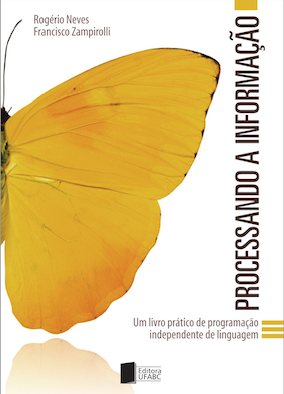
\includegraphics{"figs/Capa_Processando_Informacao.jpg"}

Este caderno (Notebook) é parte complementar \emph{online} do livro
\textbf{\href{https://editora.ufabc.edu.br/matematica-e-ciencias-da-computacao/58-processando-a-informacao}{Processando
a Informação}: um livro prático de programação independente de
linguagem}, que deve ser consultado no caso de dúvidas sobre os temas
apresentados.

\begin{quote}
Este conteúdo pode ser copiado e alterado livremente e foi inspirado
nesse livro.
\end{quote}

\begin{quote}
O conteúdo deste capítulo foi inspirado em: *
\href{https://www.ime.usp.br/~pf/algoritmos/aulas/pont.html}{Notas do
prof. Paulo Feofiloff} * Notas de aula de professores da UFABC, em
especial, dos professores Luiz Rozante e Wagner Botelho.
\end{quote}

    \hypertarget{sumuxe1rio}{%
\subsection{Sumário}\label{sumuxe1rio}}

\begin{itemize}
\tightlist
\item
  Revisão do capítulo anterior
\item
  Introdução
\item
\item
  Revisão deste capítulo
\item
  Exercícios
\end{itemize}

    \hypertarget{revisuxe3o-do-capuxedtulo-anterior-struct}{%
\subsection{Revisão do capítulo anterior
(Struct)}\label{revisuxe3o-do-capuxedtulo-anterior-struct}}

    \begin{itemize}
\tightlist
\item
  Introdução
\item
  Paradigma Estruturado
\item
  Paradigma Orientado a Objetos
\item
  Tipos de dados
\item
  Arquivos
\item
  Revisão deste capítulo
\item
  Exercícios
\end{itemize}

    \hypertarget{introduuxe7uxe3o}{%
\subsection{Introdução}\label{introduuxe7uxe3o}}

    \begin{itemize}
\item
  \emph{Ponteiros} são variáveis especiais que recebem valores
  referentes à \emph{endereços} da memória principal do computador (RAM
  - \emph{Random Access Memory}).
\item
  Ao ligar um computador, o sistema operacional é carregado da memória
  secundária para a RAM.
\item
  Quando criamos um programa em alguma linguagem de programação e
  executamos, esse programa também é carregado na RAM.
\item
  Uma variável \texttt{x=10} criada nesse programa também será
  enderaçada na RAM, por exemplo, no endereço \texttt{FF10AF} (em
  hexadecimal).
\item
  Algumas linguagens de programação aceitam também essas variáveis
  especiais do tipo \emph{ponteiros}. Por exemplo, em C podemos criar
  \texttt{int\ *p=FF10AF}.
\item
  Em geral, não precisamos saber qual é o endereço de memória de uma
  variável, mas é importante saber associar a um ponteiro. Por exemplo,
  a seguir é criada uma variável inteira \texttt{x=10} e em seguida um
  ponteiro \texttt{p} é associado a \texttt{x}, incluindo um prefixo
  \texttt{\&}, para pegar o endereço de memória de \texttt{x} e associar
  a \texttt{p}, com \texttt{p\ =\ \&x}. Para alterar o conteúdo de
  \texttt{p} (o mesmo de \texttt{x}), bastar incluir o prefixo
  \texttt{*}, ou seja, \texttt{*p\ =\ 15}. Ver também a figura a seguir
  para melhor visualizar operações com ponteiros.
\end{itemize}

\begin{verbatim}
  int x = 10;
  int *p;     // cria um ponteiro para um inteiro
  p = &x;     // faz p apontar para o endereço de x
  *p = 15;    // altera o conteúdo de p (e também de x)
  printf("x=%d *p=%d", x, *p);
\end{verbatim}

    \hypertarget{alocauxe7uxe3o-estuxe1tica}{%
\subsection{Alocação estática}\label{alocauxe7uxe3o-estuxe1tica}}

    \begin{itemize}
\tightlist
\item
  A \emph{alocação estática} ocorre em \emph{tempo de compilação} a
  depender a linguagem de programação escolhida. Por exemplo, no exemplo
  a seguir, o vetor \texttt{v} é criado contendo 3 elementos inteiros.
  Não é possível incluir um quarto elemento nesse vetor quando
  executamos o progroma (ou seja, em \emph{tempo de execução}).
\item
  Ao criar vetores ou matrizes, estamos criando ponteiros para o
  primeiro elemento dessas estruturas. Por exemplo,
\end{itemize}

\begin{verbatim}
  int v[3] = { 5,6,7 };
  int* p1;
  p1 = v; // observe que aqui não precisa usar &v
  for (int i = 0; i < 3; i++)
    printf("%d %d %d\n", *(p1 + i), p1[i], v[i]); // *(p1+i) = p1[i] = v[i]
\end{verbatim}

\begin{itemize}
\item
  Assim, nesse exemplo é possível fazer operações de ponteiros
  (\texttt{p1\ +\ i}) para acessar os endereços
  \texttt{p1,\ p1+1,\ p1+2,} \$\cdots \$
\item
  Para a variável ponteiro do tipo \emph{char}, \texttt{char\ *p} ocupa
  um \emph{byte}. Para \emph{int} são 4 \emph{bytes} e para
  \emph{double} são 8 \emph{bytes}, a dependendo da arquitetura do
  computador.
\item
  Para saber a quantidade de bytes que uma variável ocupa, usar a função
  \texttt{sizeof}.
\item
  Por exemplo, para uma variável do tipo \texttt{double} ocupa, basta
  fazer \texttt{sizeof\ (double)}, ou \texttt{sizeof(p1)}, onde
  \texttt{p1} foi definido no anterior.
\item
  Também é possível calcular o tamanho de um vetor em tempo de execução.
  Para o exemplo anterior, basta fazer:
  \texttt{sizeof(v)\ /\ sizeof(int)}.
\item
  Esse cálculo é útil para saber o tamanho de um \emph{array} definido
  em tempo de execução (\emph{alocação dinâmica} - ver próxima seção).
\end{itemize}

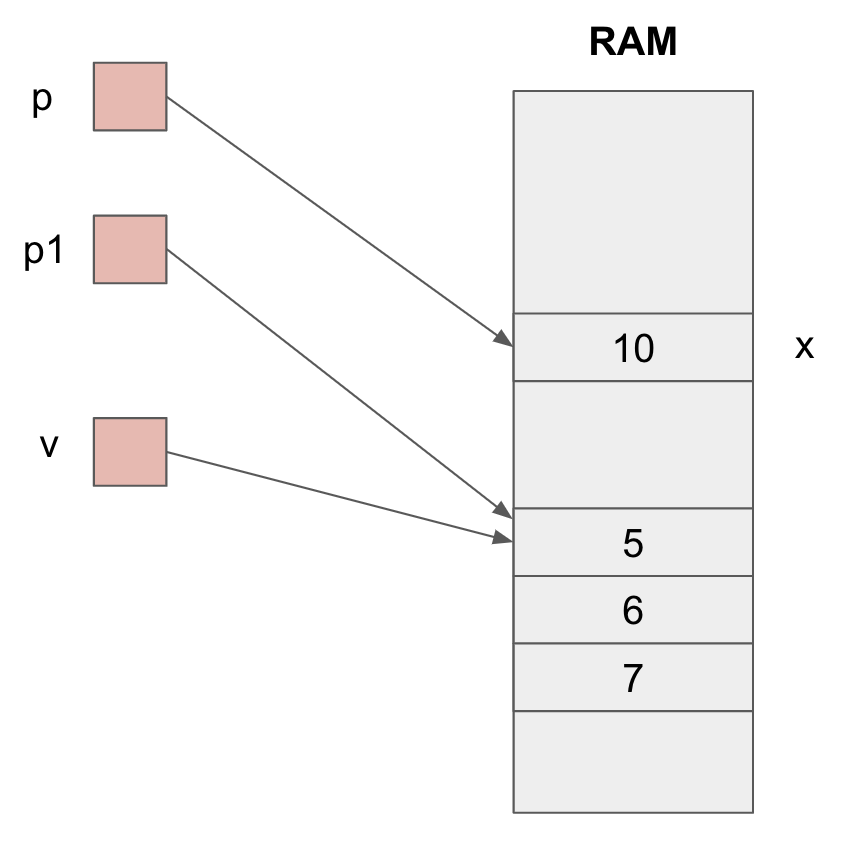
\includegraphics{"figs/cap8_1.png"}

    \begin{figure}
\centering
\caption{cap8\_1.png}
\end{figure}

    \begin{itemize}
\tightlist
\item
  Também é possível fazer operações de ponteiros para \emph{array} de
  \texttt{struct}. Ver um exemplo a seguir:
\end{itemize}

    \hypertarget{exemplo-01---criar-um-registro-de-aluno-com-scanf}{%
\subsubsection{\texorpdfstring{Exemplo 01 - Criar um registro de Aluno,
com
\texttt{scanf}}{Exemplo 01 - Criar um registro de Aluno, com scanf}}\label{exemplo-01---criar-um-registro-de-aluno-com-scanf}}

Exemplo para criar um \emph{array} de \texttt{struct} \textbf{Aluno}
contendo 4 atributos lidos do teclado com \texttt{scanf}. Associar um
ponteiro para essa \texttt{struct}.

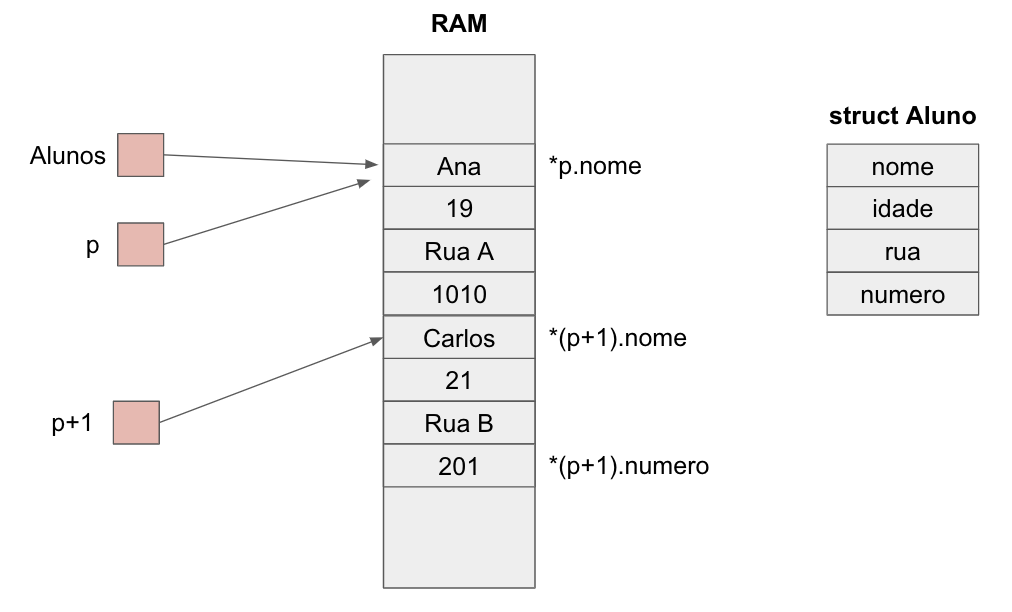
\includegraphics{"figs/cap8_2.png"}

    \begin{figure}
\centering
\caption{cap8\_2.png}
\end{figure}

    \begin{tcolorbox}[breakable, size=fbox, boxrule=1pt, pad at break*=1mm,colback=cellbackground, colframe=cellborder]
\prompt{In}{incolor}{ }{\boxspacing}
\begin{Verbatim}[commandchars=\\\{\}]
\PY{o}{\PYZpc{}\PYZpc{}writefile} cap8ex01.c
\PY{c+c1}{\PYZsh{}include \PYZlt{}stdio.h\PYZgt{}}
\PY{c+c1}{\PYZsh{}include \PYZlt{}string.h\PYZgt{}}

\PY{n}{typedef} \PY{n}{struct} \PY{p}{\PYZob{}}
  \PY{n}{char} \PY{n}{nome}\PY{p}{[}\PY{l+m+mi}{50}\PY{p}{]}\PY{p}{;}
  \PY{n+nb}{int} \PY{n}{idade}\PY{p}{;}
  \PY{n}{char} \PY{n}{rua}\PY{p}{[}\PY{l+m+mi}{50}\PY{p}{]}\PY{p}{;}
  \PY{n+nb}{int} \PY{n}{numero}\PY{p}{;}
\PY{p}{\PYZcb{}} \PY{n}{Aluno}\PY{p}{;}

\PY{n+nb}{int} \PY{n}{main}\PY{p}{(}\PY{p}{)} \PY{p}{\PYZob{}}
  \PY{n}{Aluno} \PY{n}{Alunos}\PY{p}{[}\PY{l+m+mi}{2}\PY{p}{]}\PY{p}{;} \PY{o}{/}\PY{o}{/} \PY{n}{instancia} \PY{n}{uma} \PY{n}{vetor} \PY{n}{do} \PY{n}{tipo} \PY{n}{Aluno}
  \PY{n}{Aluno} \PY{o}{*}\PY{n}{p}\PY{p}{;} \PY{o}{/}\PY{o}{/} \PY{n}{cria} \PY{n}{um} \PY{n}{ponteiro} \PY{n}{para} \PY{n}{Aluno}
  \PY{n}{p} \PY{o}{=} \PY{n}{Alunos}\PY{p}{;} \PY{o}{/}\PY{o}{/} \PY{n}{ATENÇÃO}\PY{p}{:} \PY{n}{associa} \PY{n}{p} \PY{n}{a} \PY{n}{array} \PY{n}{de} \PY{n}{alunos}
  \PY{o}{/}\PY{o}{/} \PY{n}{ENTRADA} \PY{n}{DE} \PY{n}{DADOS}
  \PY{k}{for} \PY{p}{(}\PY{n+nb}{int} \PY{n}{i} \PY{o}{=} \PY{l+m+mi}{0}\PY{p}{;} \PY{n}{i} \PY{o}{\PYZlt{}} \PY{l+m+mi}{2}\PY{p}{;} \PY{n}{i}\PY{o}{+}\PY{o}{+}\PY{p}{)} \PY{p}{\PYZob{}}
    \PY{n}{printf}\PY{p}{(}\PY{l+s+s2}{\PYZdq{}}\PY{l+s+s2}{Entre com os dados: nome, idade, rua, número:}\PY{l+s+se}{\PYZbs{}n}\PY{l+s+s2}{\PYZdq{}}\PY{p}{)}\PY{p}{;}
    \PY{n}{fflush}\PY{p}{(}\PY{n}{stdin}\PY{p}{)}\PY{p}{;}
    \PY{n}{fgets}\PY{p}{(}\PY{n}{p}\PY{p}{[}\PY{n}{i}\PY{p}{]}\PY{o}{.}\PY{n}{nome}\PY{p}{,} \PY{l+m+mi}{50}\PY{p}{,} \PY{n}{stdin}\PY{p}{)}\PY{p}{;}
    \PY{n}{scanf}\PY{p}{(}\PY{l+s+s2}{\PYZdq{}}\PY{l+s+si}{\PYZpc{}d}\PY{l+s+s2}{\PYZdq{}}\PY{p}{,} \PY{o}{\PYZam{}}\PY{n}{p}\PY{p}{[}\PY{n}{i}\PY{p}{]}\PY{o}{.}\PY{n}{idade}\PY{p}{)}\PY{p}{;}
    \PY{n}{fflush}\PY{p}{(}\PY{n}{stdin}\PY{p}{)}\PY{p}{;}
    \PY{n}{fgets}\PY{p}{(}\PY{n}{p}\PY{p}{[}\PY{n}{i}\PY{p}{]}\PY{o}{.}\PY{n}{rua}\PY{p}{,} \PY{l+m+mi}{50}\PY{p}{,} \PY{n}{stdin}\PY{p}{)}\PY{p}{;}
    \PY{n}{scanf}\PY{p}{(}\PY{l+s+s2}{\PYZdq{}}\PY{l+s+si}{\PYZpc{}d}\PY{l+s+s2}{\PYZdq{}}\PY{p}{,} \PY{o}{\PYZam{}}\PY{n}{p}\PY{p}{[}\PY{n}{i}\PY{p}{]}\PY{o}{.}\PY{n}{numero}\PY{p}{)}\PY{p}{;}
  \PY{p}{\PYZcb{}}
  \PY{o}{/}\PY{o}{/} \PY{n}{SAÍDA} \PY{n}{DE} \PY{n}{DADOS}
  \PY{k}{for} \PY{p}{(}\PY{n+nb}{int} \PY{n}{i} \PY{o}{=} \PY{l+m+mi}{0}\PY{p}{;} \PY{n}{i} \PY{o}{\PYZlt{}} \PY{l+m+mi}{2}\PY{p}{;} \PY{n}{i}\PY{o}{+}\PY{o}{+}\PY{p}{)} \PY{p}{\PYZob{}}
    \PY{n}{printf}\PY{p}{(}\PY{l+s+s2}{\PYZdq{}}\PY{l+s+s2}{nome: }\PY{l+s+si}{\PYZpc{}s}\PY{l+s+se}{\PYZbs{}n}\PY{l+s+s2}{idade: }\PY{l+s+si}{\PYZpc{}d}\PY{l+s+se}{\PYZbs{}n}\PY{l+s+s2}{\PYZdq{}}\PY{p}{,} \PY{n}{p}\PY{p}{[}\PY{n}{i}\PY{p}{]}\PY{o}{.}\PY{n}{nome}\PY{p}{,} \PY{n}{p}\PY{p}{[}\PY{n}{i}\PY{p}{]}\PY{o}{.}\PY{n}{idade}\PY{p}{)}\PY{p}{;}
    \PY{n}{printf}\PY{p}{(}\PY{l+s+s2}{\PYZdq{}}\PY{l+s+s2}{rua: }\PY{l+s+si}{\PYZpc{}s}\PY{l+s+se}{\PYZbs{}n}\PY{l+s+s2}{número: }\PY{l+s+si}{\PYZpc{}d}\PY{l+s+se}{\PYZbs{}n}\PY{l+s+s2}{\PYZdq{}}\PY{p}{,} \PY{n}{p}\PY{p}{[}\PY{n}{i}\PY{p}{]}\PY{o}{.}\PY{n}{rua}\PY{p}{,} \PY{n}{p}\PY{p}{[}\PY{n}{i}\PY{p}{]}\PY{o}{.}\PY{n}{numero}\PY{p}{)}\PY{p}{;}
  \PY{p}{\PYZcb{}}
  \PY{k}{return} \PY{l+m+mi}{0}\PY{p}{;}
\PY{p}{\PYZcb{}}
\end{Verbatim}
\end{tcolorbox}

    \begin{tcolorbox}[breakable, size=fbox, boxrule=1pt, pad at break*=1mm,colback=cellbackground, colframe=cellborder]
\prompt{In}{incolor}{ }{\boxspacing}
\begin{Verbatim}[commandchars=\\\{\}]
\PY{o}{\PYZpc{}\PYZpc{}}\PY{k}{shell}
gcc \PYZhy{}Wall \PYZhy{}std=c99 cap8ex01.c \PYZhy{}o output
./output
\end{Verbatim}
\end{tcolorbox}

    \hypertarget{alocauxe7uxe3o-dinuxe2mica}{%
\subsection{Alocação dinâmica}\label{alocauxe7uxe3o-dinuxe2mica}}

    \begin{itemize}
\item
  A alocação dinâmica ocorre quando não sabemos o tamanho de um
  \emph{array} em tempo de compilação, sendo necessário alocar em tempo
  de execução.
\item
  Até agora utilizamos alocação estática para definir o tamanho de um
  \emph{array}. Por exemplo, para criar um \emph{array} de alunos da
  UFABC, podemos criar um \emph{array} ``muito grande'', por exemplo,
  contendo 100000 alunos.
\item
  Nesse caso, temos dois problemas, se um dia tivermos mais que 100000
  alunos, esse \emph{array} não vai suportar.
\item
  O outro problema é que em geral estamos desperdiçando memória RAM com
  as posição do \emph{array} não utilizadas.
\item
  Para resolver isso, utilizamos \emph{alocação dinâmica}, inserindo ou
  retirando elementos do \emph{array} conforme a demanda.
\item
  Na linguagem C existem os seguintes comandos da biblioteca
  \texttt{stdlib.h}:

  \begin{itemize}
  \tightlist
  \item
    \texttt{malloc}

    \begin{itemize}
    \tightlist
    \item
      sintaxe:
      \texttt{int\ *\ p\ =\ (int\ *)\ malloc(\ TAMANHO\ *\ sizeof(int)\ )}
    \item
      comando utilizado para alocar um \emph{array} de \texttt{TAMANHO}
      de inteiros.
    \item
      O ponteiro \texttt{p} aponta para o primeiro elemento do
      \emph{array}.
    \item
      É possível definir um \emph{array} para qualquer tipo de dado,
      inclusive para \texttt{struct}.
    \item
      Se \texttt{p\ =\ NULL} então não existe memória suficiente para a
      alocação.
    \end{itemize}
  \item
    \texttt{calloc}

    \begin{itemize}
    \tightlist
    \item
      sintaxe:
      \texttt{int\ *\ p\ =\ (int\ *)\ calloc(\ TAMANHO,\ \ sizeof(int)\ )}
    \item
      análogo ao \texttt{malloc}, porém com \texttt{calloca} possui dois
      argumentos e inicializa todos os elementos com 0s.
    \end{itemize}
  \item
    \texttt{realloc}

    \begin{itemize}
    \tightlist
    \item
      sintaxe:
      \texttt{int\ *\ p\ =\ (int\ *)\ realloc(\ TAMANHO,\ \ sizeof(int)\ )}
    \item
      realoca um \emph{array}
    \end{itemize}
  \item
    \texttt{free}

    \begin{itemize}
    \tightlist
    \item
      sempre que alocamos memória dinâmicamente devemos liberar a
      memória no final, com o camando \texttt{free(p)}.
    \item
      se isso não for feito, a memória será liberada somente quando o
      computador for desligado (se o sistema operacional não tiver algum
      recurso de ``coleta de lixo'').
    \end{itemize}
  \end{itemize}
\end{itemize}

    \hypertarget{exemplo-de-alocauxe7uxe3o-estuxe1tica}{%
\subsubsection{Exemplo de alocação
estática}\label{exemplo-de-alocauxe7uxe3o-estuxe1tica}}

\begin{verbatim}
void main(){
    int TAMANHO = 0;
    scanf("%i", &TAMANHO);
    int v[TAMANHO]; // NÃO PODE ALTER O TAMANHO APÓS CRIADO!!!
    // free(v); // LOGO, NÃO PODE USAR free!!!
}
\end{verbatim}

    \hypertarget{exemplo-de-alocauxe7uxe3o-dinuxe2mica}{%
\subsubsection{Exemplo de alocação
dinâmica}\label{exemplo-de-alocauxe7uxe3o-dinuxe2mica}}

\begin{verbatim}
void main(){
    int TAMANHO = 0;
    scanf("%i", &TAMANHO);
    int *v = (int *) malloc( TAMANHO * sizeof(int) );
    free(v); // LIBERAR A MEMÓRIA - S E M P R E !!!!
}
\end{verbatim}

    \hypertarget{alocauxe7uxe3o-dinuxe2mica-para-array-multidimensional}{%
\subsection{\texorpdfstring{Alocação dinâmica para \emph{array}
multidimensional}{Alocação dinâmica para array multidimensional}}\label{alocauxe7uxe3o-dinuxe2mica-para-array-multidimensional}}

    \begin{itemize}
\tightlist
\item
  Para utilizarmos matrizes com alocação dinâmica é interessante
  trabalharmos com \emph{ponteiro para ponteiro}:

  \begin{itemize}
  \item
    primeiro alocamos memória para as linhas (L) da matriz:

    \begin{itemize}
    \tightlist
    \item
      \texttt{int\ **m\ =\ (int**)\ malloc(\ L\ *\ sizeof(int\ *)\ );}
    \end{itemize}
  \item
    em seguida alocamos memória para cada linha da matriz (colunas C):

\begin{verbatim}
  for (int i=0; i < L; i++) 
    m[i] = (int*) malloc( C * sizeof(int *) ); // m[i] = *(m+i)
\end{verbatim}
  \item
    para popular a matriz - opção 1:

\begin{verbatim}
  for (int i=0; i < L; i++) 
    for (int j=0; j < C; J++) 
      scanf("%d", &m[i][j]); // &m[i][j] = m + i*C + j
\end{verbatim}
  \item
    para popular a matriz - opção 2:

\begin{verbatim}
  for (int i=0; i < L*C; i++) 
      scanf("%d", m+i); // m+i = &m[i/C][i%C]
\end{verbatim}
  \item
    não esquecer de LIBERAR A MEMÓRIA:

    \begin{itemize}
    \tightlist
    \item
      primeiro o conteúdo de cada linha:
    \end{itemize}

\begin{verbatim}
  for (int i=0; i < L; i++) 
    free(m[i]); // m[i] = *(m+i)
\end{verbatim}

    \begin{itemize}
    \tightlist
    \item
      depois toda a matriz:
    \end{itemize}

\begin{verbatim}
free(m);
\end{verbatim}
  \end{itemize}
\end{itemize}

    \hypertarget{exemplo-01---lerescrever-matriz-com-muxe9todos-cap.6---matriz}{%
\subsection{Exemplo 01 - Ler/Escrever matriz com métodos (cap.6 -
Matriz)}\label{exemplo-01---lerescrever-matriz-com-muxe9todos-cap.6---matriz}}

    \begin{itemize}
\item
  Analogamente ao que foi feito no capítulo sobre vetores, onde alocamos
  os vetores em tempo de execução através de métodos, é possível usar
  modularização para melhorar a organização, manutenção e
  reaproveitamento de código.
\item
  Aqui é apresentado um método \texttt{leiaMatriz} e
  \texttt{escrevaMatriz} genéricos
\item
  Para entrada de dados, ou seja, inserir valores nos elementos alocados
  na memória para uma matriz.
\item
  Além de saída de dados, para escrever a matriz, linha por linha.
\end{itemize}

    \hypertarget{pseudocuxf3digo}{%
\paragraph{Pseudocódigo}\label{pseudocuxf3digo}}

    \textbf{Exemplo 01:} Considere um algoritmo para: * Ler um inteiro
\texttt{L} (linhas) representando o número de alunos, * Ler um inteiro
\texttt{C} representando o número de avaliações. * Considere a primeira
coluna o \texttt{RA} do aluno, assim \texttt{C=C+1}. * Criar uma matriz
\texttt{m} com dimensões \texttt{LxC}. * Ler todos os elementos da
matriz. * Escrever todos os elementos da matriz, formando a saída, linha
por linha, por exemplo, para uma matriz com \texttt{2} alunos e
\texttt{3} avaliações, escreva:

\begin{verbatim}
LISTA DE ALUNOS vs Avaliações:
1234 4 3 9
3456 6 4 8
\end{verbatim}

    \begin{verbatim}
Função inteiro m[][] leiaMatriz(inteiro L, inteiro C):
    Instanciar e alocar uma matriz m de Reais com L x C
    Para cada i, de i=0; até i<L; passo i=i+1 faça
        Para cada j, de j=0; até j<C; passo j=j+1 faça
            m[i,j] = leia("Digite um número inteiro:");

Função escrevaMatriz(inteiro m[][], inteiro L, inteiro C): 
    Instanciar e alocar uma matriz m de Reais com L x C
    Para cada i, de i=0; até i<L; passo i=i+1 faça
        Para cada j, de j=0; até j<C; passo j=j+1 faça
            escreva(" ", m[i,j]);
        escreva("\n"); // pula linha

// PROGRAMA PRINCIPAL
// ENTRADAS
inteiro L = leia("Digite o numero de alunos:")
inteiro C = leia("Digite o numero de avaliações:")
C = C + 1  // a primeira coluna é o RA
Instanciar uma matriz m com L linhas e C colunas 

m = leiaMatriz(L,C)
// PROCESSAMENTO: ?

// SAÍDA
escrevaMatriz(m)
\end{verbatim}

    \hypertarget{casos-para-teste-moodlevpl}{%
\paragraph{Casos para Teste
Moodle+VPL}\label{casos-para-teste-moodlevpl}}

Para o professor criar uma atividade VPL no Moodle para este Exemplo 01,
basta incluir em \texttt{Casos\ para\ teste}, o seguinte texto (pode
incluir mais casos):

\begin{verbatim}
case=caso1
input=2
3
1234 
4 
3 
9
3456
6
4
8
output=
LISTA DE ALUNOS vs Avaliações:
1234 4 3 9
3456 6 4 8
\end{verbatim}

    \begin{tcolorbox}[breakable, size=fbox, boxrule=1pt, pad at break*=1mm,colback=cellbackground, colframe=cellborder]
\prompt{In}{incolor}{ }{\boxspacing}
\begin{Verbatim}[commandchars=\\\{\}]
\PY{o}{\PYZpc{}\PYZpc{}writefile} cap8ex02.c
\PY{c+c1}{\PYZsh{}include \PYZlt{}stdio.h\PYZgt{}}
\PY{c+c1}{\PYZsh{}include\PYZlt{}malloc.h\PYZgt{}  }

\PY{n+nb}{int} \PY{o}{*}\PY{o}{*} \PY{n}{leiaMatriz}\PY{p}{(}\PY{n+nb}{int} \PY{n}{L}\PY{p}{,} \PY{n+nb}{int} \PY{n}{C}\PY{p}{)} \PY{p}{\PYZob{}}
  \PY{n+nb}{int} \PY{o}{*}\PY{o}{*}\PY{n}{m} \PY{o}{=} \PY{p}{(}\PY{n+nb}{int} \PY{o}{*}\PY{o}{*}\PY{p}{)}\PY{n}{malloc}\PY{p}{(}\PY{n}{L}\PY{o}{*}\PY{n}{sizeof}\PY{p}{(}\PY{n+nb}{int}\PY{o}{*}\PY{p}{)}\PY{p}{)}\PY{p}{;} 
  \PY{k}{for} \PY{p}{(}\PY{n+nb}{int} \PY{n}{i} \PY{o}{=} \PY{l+m+mi}{0}\PY{p}{;} \PY{n}{i} \PY{o}{\PYZlt{}} \PY{n}{L}\PY{p}{;} \PY{n}{i}\PY{o}{+}\PY{o}{+}\PY{p}{)} \PY{p}{\PYZob{}}
    \PY{n}{m}\PY{p}{[}\PY{n}{i}\PY{p}{]} \PY{o}{=} \PY{p}{(}\PY{n+nb}{int} \PY{o}{*}\PY{p}{)}\PY{n}{malloc}\PY{p}{(}\PY{n}{C} \PY{o}{*} \PY{n}{sizeof}\PY{p}{(}\PY{n+nb}{int}\PY{p}{)}\PY{p}{)}\PY{p}{;} \PY{o}{/}\PY{o}{/} \PY{k}{for} \PY{n}{each} \PY{n}{row} \PY{n}{allocate} \PY{n}{C} \PY{n}{ints}
    \PY{k}{for} \PY{p}{(}\PY{n+nb}{int} \PY{n}{j} \PY{o}{=} \PY{l+m+mi}{0}\PY{p}{;} \PY{n}{j} \PY{o}{\PYZlt{}} \PY{n}{C}\PY{p}{;} \PY{n}{j}\PY{o}{+}\PY{o}{+}\PY{p}{)} 
      \PY{n}{scanf}\PY{p}{(}\PY{l+s+s2}{\PYZdq{}}\PY{l+s+si}{\PYZpc{}d}\PY{l+s+s2}{\PYZdq{}}\PY{p}{,} \PY{o}{\PYZam{}}\PY{n}{m}\PY{p}{[}\PY{n}{i}\PY{p}{]}\PY{p}{[}\PY{n}{j}\PY{p}{]}\PY{p}{)}\PY{p}{;} 
  \PY{p}{\PYZcb{}}
  \PY{k}{return} \PY{n}{m}\PY{p}{;}
\PY{p}{\PYZcb{}}
\PY{n}{void} \PY{n}{free\PYZus{}matrix}\PY{p}{(}\PY{n+nb}{int} \PY{o}{*}\PY{o}{*}\PY{n}{m}\PY{p}{,} \PY{n+nb}{int} \PY{n}{L}\PY{p}{)} \PY{p}{\PYZob{}}
    \PY{k}{for} \PY{p}{(}\PY{n+nb}{int} \PY{n}{i} \PY{o}{=} \PY{l+m+mi}{0}\PY{p}{;} \PY{n}{i} \PY{o}{\PYZlt{}} \PY{n}{L}\PY{p}{;} \PY{n}{i}\PY{o}{+}\PY{o}{+}\PY{p}{)} 
         \PY{n}{free}\PY{p}{(}\PY{n}{m}\PY{p}{[}\PY{n}{i}\PY{p}{]}\PY{p}{)}\PY{p}{;}
    \PY{n}{free}\PY{p}{(}\PY{n}{m}\PY{p}{)}\PY{p}{;}
 \PY{p}{\PYZcb{}}
\PY{n}{void} \PY{n}{escrevaMatriz}\PY{p}{(}\PY{n+nb}{int} \PY{o}{*}\PY{o}{*}\PY{n}{m}\PY{p}{,} \PY{n+nb}{int} \PY{n}{L}\PY{p}{,} \PY{n+nb}{int} \PY{n}{C}\PY{p}{)} \PY{p}{\PYZob{}}
  \PY{k}{for} \PY{p}{(}\PY{n+nb}{int} \PY{n}{i} \PY{o}{=} \PY{l+m+mi}{0}\PY{p}{;} \PY{n}{i} \PY{o}{\PYZlt{}} \PY{n}{L}\PY{p}{;} \PY{n}{i}\PY{o}{+}\PY{o}{+}\PY{p}{)} \PY{p}{\PYZob{}}
   \PY{k}{for} \PY{p}{(}\PY{n+nb}{int} \PY{n}{j} \PY{o}{=} \PY{l+m+mi}{0}\PY{p}{;} \PY{n}{j} \PY{o}{\PYZlt{}} \PY{n}{C}\PY{p}{;} \PY{n}{j}\PY{o}{+}\PY{o}{+}\PY{p}{)} 
      \PY{n}{printf}\PY{p}{(}\PY{l+s+s2}{\PYZdq{}}\PY{l+s+si}{\PYZpc{}d}\PY{l+s+se}{\PYZbs{}t}\PY{l+s+s2}{\PYZdq{}}\PY{p}{,} \PY{n}{m}\PY{p}{[}\PY{n}{i}\PY{p}{]}\PY{p}{[}\PY{n}{j}\PY{p}{]}\PY{p}{)}\PY{p}{;} 
   \PY{n}{printf}\PY{p}{(}\PY{l+s+s2}{\PYZdq{}}\PY{l+s+se}{\PYZbs{}n}\PY{l+s+s2}{\PYZdq{}}\PY{p}{)}\PY{p}{;}
  \PY{p}{\PYZcb{}}
\PY{p}{\PYZcb{}}
\PY{n+nb}{int} \PY{n}{main}\PY{p}{(}\PY{n}{void}\PY{p}{)} \PY{p}{\PYZob{}}
  \PY{o}{/}\PY{o}{/} \PY{n}{ENTRADA} \PY{n}{DE} \PY{n}{DADOS}
  \PY{n+nb}{int} \PY{n}{L}\PY{p}{,} \PY{n}{C}\PY{p}{,} \PY{o}{*}\PY{o}{*}\PY{n}{m}\PY{p}{;}   \PY{o}{/}\PY{o}{/} \PY{n}{variaveis} \PY{n}{de} \PY{n}{referência} \PY{n}{m}
  \PY{n}{printf}\PY{p}{(}\PY{l+s+s2}{\PYZdq{}}\PY{l+s+s2}{Digite o número de alunos: }\PY{l+s+s2}{\PYZdq{}}\PY{p}{)}\PY{p}{;}
  \PY{n}{scanf}\PY{p}{(}\PY{l+s+s2}{\PYZdq{}}\PY{l+s+si}{\PYZpc{}d}\PY{l+s+s2}{\PYZdq{}}\PY{p}{,} \PY{o}{\PYZam{}}\PY{n}{L}\PY{p}{)}\PY{p}{;}

  \PY{n}{printf}\PY{p}{(}\PY{l+s+s2}{\PYZdq{}}\PY{l+s+s2}{Digite o número de avaliações: }\PY{l+s+s2}{\PYZdq{}}\PY{p}{)}\PY{p}{;}
  \PY{n}{scanf}\PY{p}{(}\PY{l+s+s2}{\PYZdq{}}\PY{l+s+si}{\PYZpc{}d}\PY{l+s+s2}{\PYZdq{}}\PY{p}{,} \PY{o}{\PYZam{}}\PY{n}{C}\PY{p}{)}\PY{p}{;}

  \PY{n}{C} \PY{o}{=} \PY{n}{C} \PY{o}{+} \PY{l+m+mi}{1}\PY{p}{;} \PY{o}{/}\PY{o}{/} \PY{n}{a} \PY{n}{primeira} \PY{n}{coluna} \PY{n}{é} \PY{n}{o} \PY{n}{RA} \PY{n}{do} \PY{n}{aluno}

  \PY{n}{printf}\PY{p}{(}\PY{l+s+s2}{\PYZdq{}}\PY{l+s+s2}{Digite os elementos da matriz}\PY{l+s+s2}{\PYZdq{}}\PY{p}{)}\PY{p}{;}
  \PY{n}{m} \PY{o}{=} \PY{n}{leiaMatriz}\PY{p}{(}\PY{n}{L}\PY{p}{,}\PY{n}{C}\PY{p}{)}\PY{p}{;}

  \PY{o}{/}\PY{o}{/} \PY{n}{PROCESSAMENTO} \PY{err}{?}

  \PY{o}{/}\PY{o}{/} \PY{n}{SAÍDA} \PY{n}{DE} \PY{n}{DADOS}
  \PY{n}{printf}\PY{p}{(}\PY{l+s+s2}{\PYZdq{}}\PY{l+s+se}{\PYZbs{}n}\PY{l+s+s2}{LISTA DE ALUNOS vs Avaliações:}\PY{l+s+se}{\PYZbs{}n}\PY{l+s+s2}{\PYZdq{}}\PY{p}{)}\PY{p}{;}
  \PY{n}{printf}\PY{p}{(}\PY{l+s+s2}{\PYZdq{}}\PY{l+s+s2}{RA }\PY{l+s+s2}{\PYZdq{}}\PY{p}{)}\PY{p}{;}
  \PY{k}{for} \PY{p}{(}\PY{n+nb}{int} \PY{n}{i} \PY{o}{=} \PY{l+m+mi}{0}\PY{p}{;} \PY{n}{i} \PY{o}{\PYZlt{}} \PY{n}{C}\PY{o}{\PYZhy{}}\PY{l+m+mi}{1}\PY{p}{;} \PY{n}{i}\PY{o}{+}\PY{o}{+}\PY{p}{)} 
    \PY{n}{printf}\PY{p}{(}\PY{l+s+s2}{\PYZdq{}}\PY{l+s+se}{\PYZbs{}t}\PY{l+s+si}{\PYZpc{}d}\PY{l+s+s2}{\PYZdq{}}\PY{p}{,}\PY{p}{(}\PY{n}{i}\PY{o}{+}\PY{l+m+mi}{1}\PY{p}{)}\PY{p}{)}\PY{p}{;} 
  
  \PY{n}{printf}\PY{p}{(}\PY{l+s+s2}{\PYZdq{}}\PY{l+s+se}{\PYZbs{}n}\PY{l+s+s2}{\PYZdq{}}\PY{p}{)}\PY{p}{;}
  \PY{n}{escrevaMatriz}\PY{p}{(}\PY{n}{m}\PY{p}{,}\PY{n}{L}\PY{p}{,}\PY{n}{C}\PY{p}{)}\PY{p}{;}
  \PY{n}{free\PYZus{}matrix}\PY{p}{(}\PY{n}{m}\PY{p}{,}\PY{n}{L}\PY{p}{)}\PY{p}{;} \PY{o}{/}\PY{o}{/} \PY{n}{liberar} \PY{n}{memória} \PY{n}{alocado} \PY{n}{com} \PY{n}{malloc}
  \PY{k}{return} \PY{l+m+mi}{0}\PY{p}{;}
\PY{p}{\PYZcb{}}
\end{Verbatim}
\end{tcolorbox}

    \begin{tcolorbox}[breakable, size=fbox, boxrule=1pt, pad at break*=1mm,colback=cellbackground, colframe=cellborder]
\prompt{In}{incolor}{ }{\boxspacing}
\begin{Verbatim}[commandchars=\\\{\}]
\PY{o}{\PYZpc{}\PYZpc{}}\PY{k}{shell}
gcc \PYZhy{}Wall \PYZhy{}std=c99 cap8ex02.c \PYZhy{}o output
./output
\end{Verbatim}
\end{tcolorbox}

    \hypertarget{acessando-elemento-com}{%
\subparagraph{\texorpdfstring{Acessando elemento com
\texttt{*}}{Acessando elemento com *}}\label{acessando-elemento-com}}

Outras forma de acessar elementos em matriz.

\begin{verbatim}
  for (int i = 0; i < L; i++) 
   for (int j = 0; j < C; j++) {
      printf("%d\t", m[i][j]); // ou
      printf("%d\t", *(m + i*C + j));
   }
\end{verbatim}

Ou utilizando apenas um laço para varrar uma matriz:

\begin{verbatim}
  for (int i = 0; i < L*C; i++) {
      printf("%d\t", m[i/C][i%C]); // ou
      printf("%d\t", *(m + i));
   }
\end{verbatim}

    \hypertarget{matriz-multimensional}{%
\subparagraph{Matriz Multimensional}\label{matriz-multimensional}}

\begin{verbatim}
for (int k = 0; k < D; k++) // profundidade
  for (int i = 0; i < L; i++) // linha
   for (int j = 0; j < C; j++) { // coluna
      printf("%d\t", m[k][i][j]); // ou
      printf("%d\t", *(m + k*L*C + i*C + j));
   }
\end{verbatim}

Ou utilizando apenas um laço para varrar uma matriz:

\begin{verbatim}
  for (int i = 0; i < D*L*C; i++) {
      d = i/(L*C);
      printf("%d\t", m[d][(d-i)/C][(d-i)%C]); // ou
      printf("%d\t", *(m + i));
   }
\end{verbatim}

    \hypertarget{exercuxedcios}{%
\subsection{Exercícios}\label{exercuxedcios}}

    Ver notebook Colab nos arquivos \texttt{cap8.partX.lab.*.ipynb}
(\texttt{X} \(\in\) \texttt{{[}2,3,4,5{]}} e \texttt{*} é a extensão da
linguagem), utilizando alguma linguagem de programação de sua
preferência, onganizadas em subpastas contidas em \texttt{"gen"}, na
pasta do Google Drive
\href{https://drive.google.com/drive/folders/1YlFwv8XYN7PYYf-HwDMlkxzbmXzJw9cM?usp=sharing}{colabs}.

    \hypertarget{revisuxe3o-deste-capuxedtulo}{%
\subsection{Revisão deste capítulo}\label{revisuxe3o-deste-capuxedtulo}}

\begin{itemize}
\tightlist
\item
  Introdução
\item
  Paradigma Estruturado
\item
  Paradigma Orientado a Objetos
\item
  Tipos de dados
\item
  Arquivos
\item
  Exercícios
\item
  Revisão deste capítulo de Vetores
\end{itemize}


    % Add a bibliography block to the postdoc
    
    
    
\end{document}
